\chapter{Softwarekonzept} \label{chap:Konzept}

Der dieser Studienarbeit zu Grunde Liegende Code wurde in der letzten Studienarbeit in einer Cloud-Umgebung entwickelt. Als einfache testumgebung zur umsetzung einer Machbarkeitsstudie war dies ausreichend. 
Da in dieser Studienarbeit das Umsetzen einer Webvisualisierung der durch die FESTO \ac{cp-lab} aufgenommenen Daten im Vordergrund steht, ist es notwendig, die Software in eine lokale Umgebung zu verschieben. 
Dies ermöglicht eine bessere Kontrolle über die Entwicklungsumgebung und die verwendeten Bibliotheken. 

Zusätzlich sollen alle einstellbaren Parameter zentral aufgeführt werden. Dies ermöglicht eine einfache Konfiguration der Software und entspricht dem Stand der Technik\cite{gur_diskussion_2024} \cite{oliveira_how_2023}. 

Die Realisierung beider Aufgaben wird in diesem Kapitel beschrieben

\section{Architektur} \label{sec:architektur}

Erster Teil der Softwarearchitektur ist die Konzeption der Struktur. Die Struktur einer Software ist entscheidend für die Wartbarkeit und Erweiterbarkeit.
Im Optimalfall ist Die Struktur so aufgebaut, dass sie einfach zu verstehen und zu warten ist.

\begin{figure}[H]
    \centering
    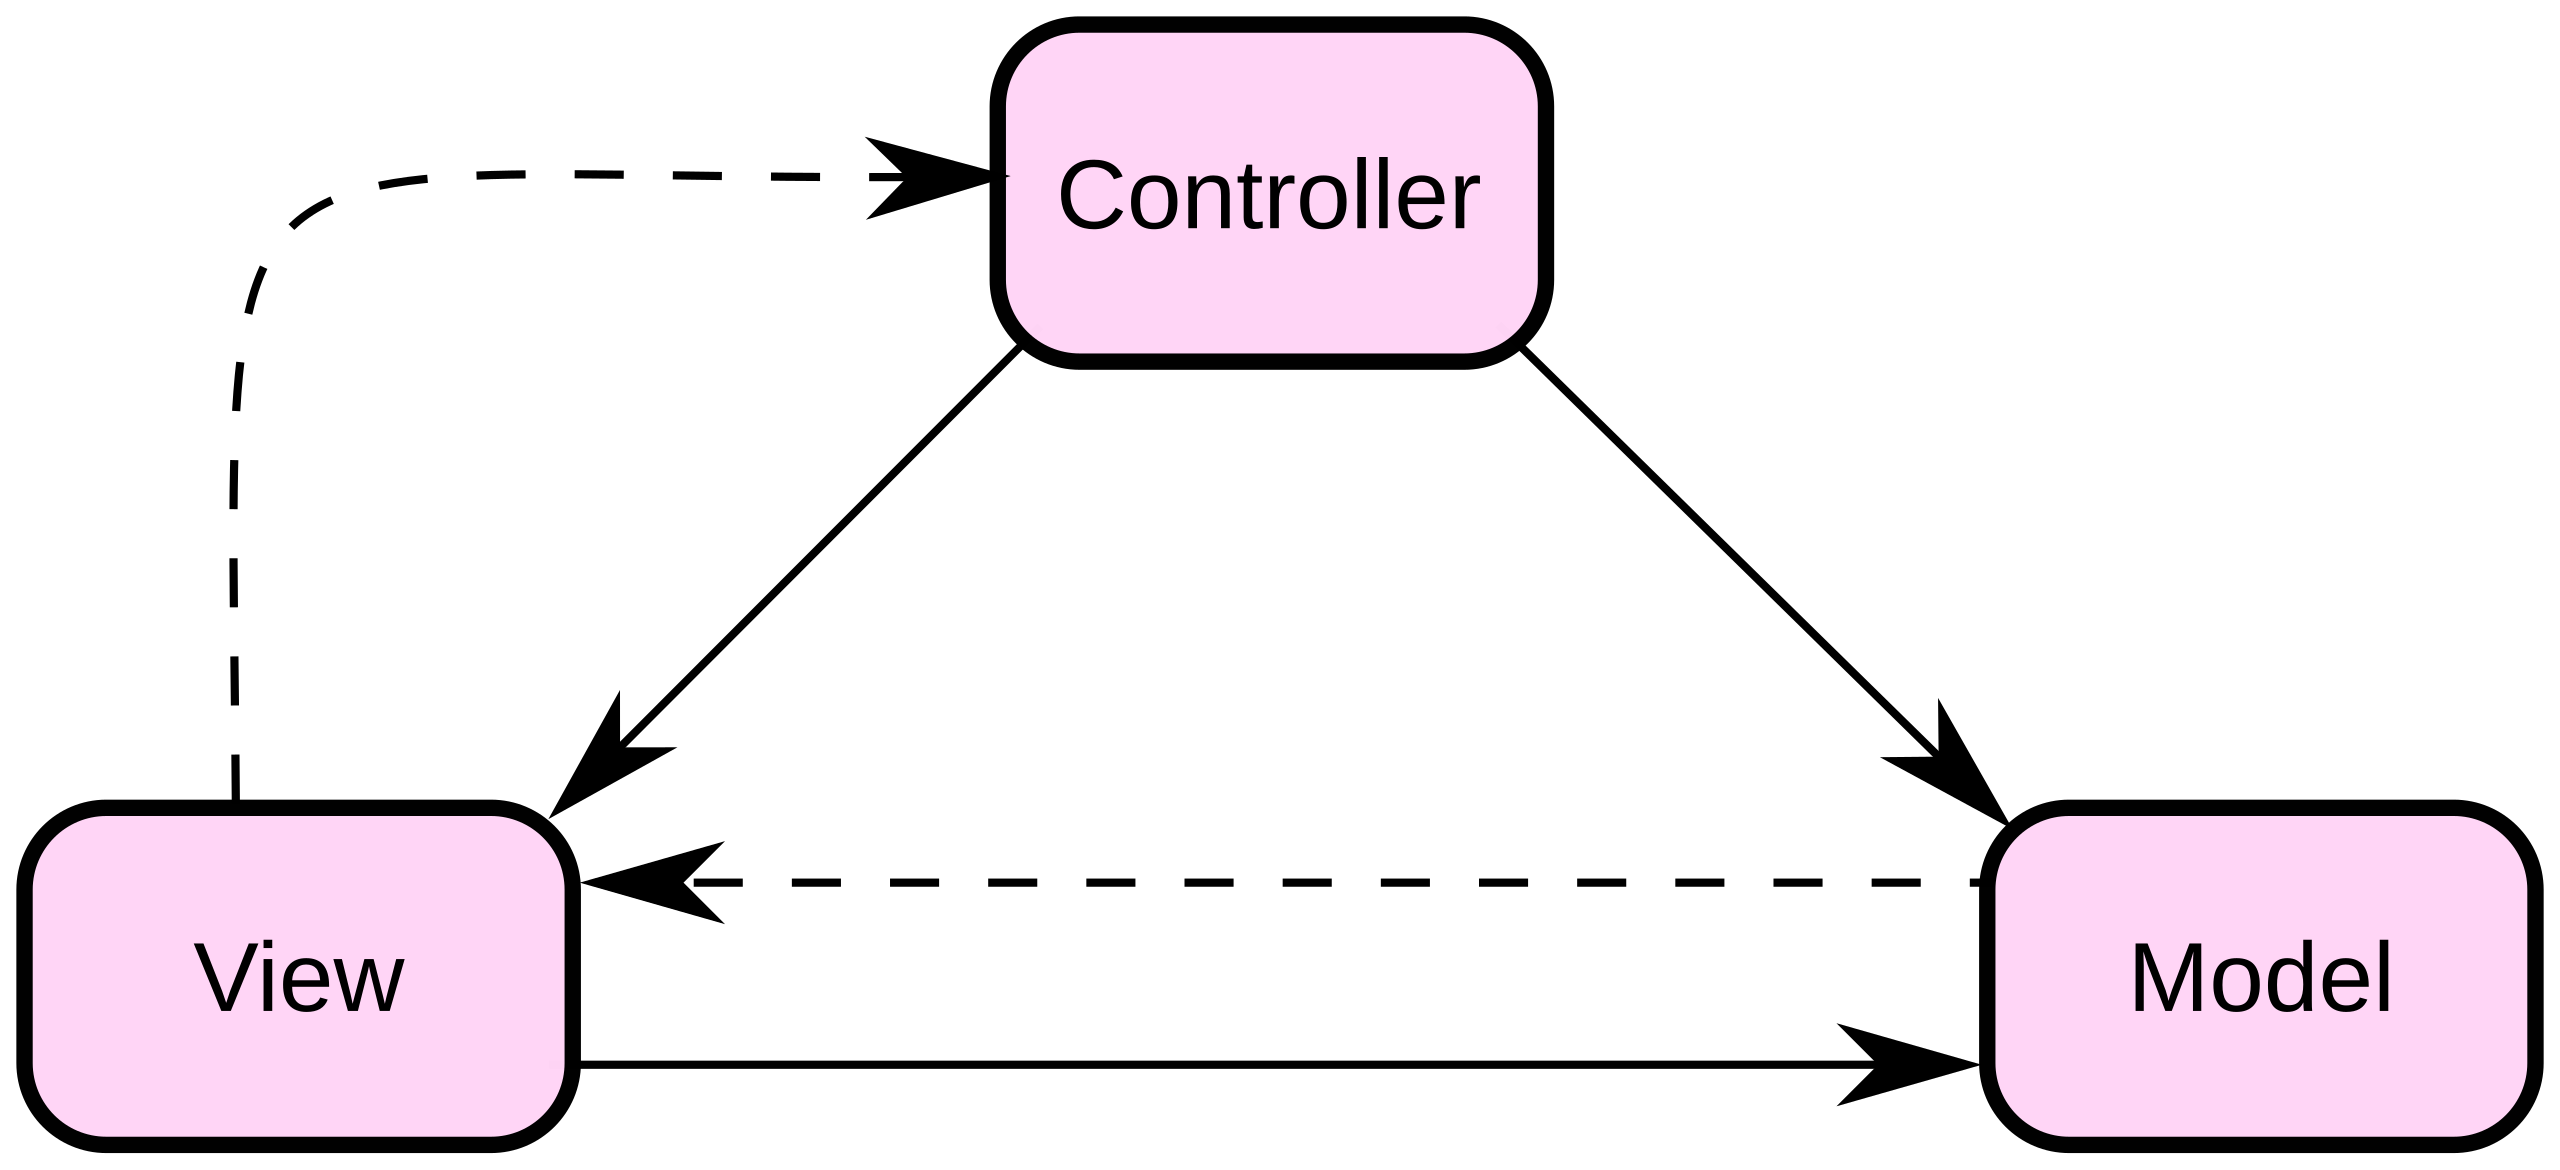
\includegraphics[width=0.8\textwidth]{MVC_struktur.png}
    \caption{Schematische Darstellung der MVC Struktur \cite{noauthor_model_2024}} 
    \label{fig:MVC_struktur}
\end{figure}

Im Rahmen dieser Studienarbeit gibt es keine externen Anforderungen an die Struktur. Daher wurde sich für eine vereinfachte \ac{MVC} Struktur entschieden (\autoref{fig:MVC_struktur}). Ziel dieser Struktur ist es die Software in drei Teile zu unterteilen.
Diese drei Teile sollen eigenständige Aufgaben übernehmen und so verhindern, dass das Programm zu einem Monolithischen Codeblock wird.

Im \ac{MVC} Modell gibt es drei Teile:
\begin{itemize}
    \item \textbf{Model}: Der Model-Teil ist für die Datenverarbeitung zuständig. Er enthält die Datenstrukturen und die Logik, die die Daten verarbeitet. 
    \item \textbf{View}: Der View-Teil ist für die Darstellung der Daten zuständig. Er enthält die Benutzeroberfläche und die Logik, die die Daten darstellt.
    \item \textbf{Controller}: Der Controller-Teil ist für die Steuerung der Daten zuständig. Er enthält die Logik, die die Daten steuert und die Kommunikation zwischen Model und View koordiniert.
\end{itemize}

Die Vereinfachte Version dieser Struktur kombiniert die Funktionalitäten von View und Controller in der API \autoref{fig:flask} und trennt die Datenverarbeitung in einem eigenen Modul, dem Pycore Modul, welches die benötigten selbst entwickelten Bibliotheken zur Verfügung stellt. 

\begin{figure}[H]
    \centering
    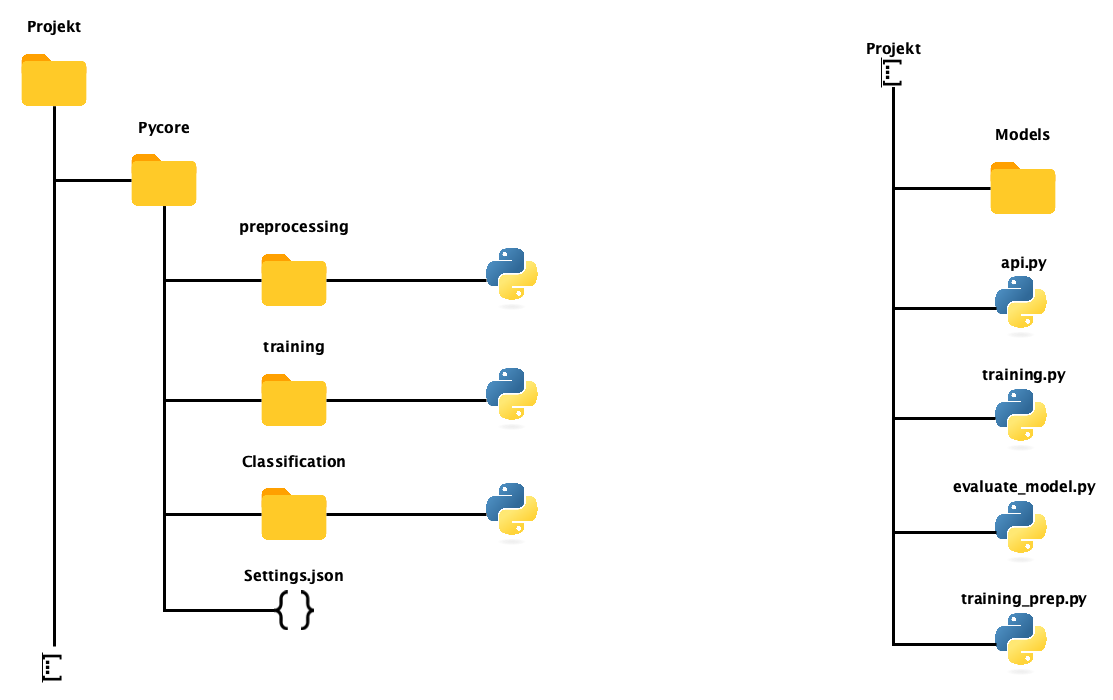
\includegraphics[width=0.8\textwidth]{Projektstruktur.png}
    \caption{Struktur der Software}
    \label{fig:Projektstruktur}
\end{figure}


\begin{lstlisting}[style=json, label=lst:json_example, caption={Beispiel einer \ac{JSON}-Datei mit Pflanzendaten}]
    {
        "filepaths": {
            "good": "Bilder/Good_Pictures",
            "bad": "Bilder/Bad_Pictures",
            "good_gray": "Bilder/Good_Grayscale",
            "bad_gray": "Bilder/Bad_Grayscale",
            "train": "Bilder/train",
            "test":"Bilder/test",
            "validate":"Bilder/validate",
            "new": "Bilder/new"
        },
        "mobilnet":{
            "weights":"imagenet",
            "include_top":false,
            "density1": 1024,
            "density2": 1024,
            "density3": 512,
            "density4": 2,
            "activation_x": "relu",
            "activation_preds": "softmax",
            "layers":20

        },
    }
\end{lstlisting}

\section{Die Weboberfläche mittels Python Web API} \label{sec:weboberflaeche}